\documentclass[11pt]{article}
\usepackage{amsmath}
\usepackage{graphicx}
\usepackage{float}
\usepackage{blindtext}
\usepackage{subcaption}
\usepackage[a4paper,margin=2cm]{geometry}
\usepackage{fancyhdr}
\usepackage{longtable}
\usepackage[
    backend=biber,
    style=ieee
]{biblatex}
\usepackage{xcolor}
\usepackage{soul}
\usepackage{listings}

\newcommand{\hlc}[2][yellow]{{%
    \colorlet{foo}{#1}%
    \sethlcolor{foo}\hl{#2}}%
}


\addbibresource{report.bib}

\graphicspath{ {./images/} }

\pagestyle{fancy}
\fancyhead[C]{Report}
\fancyhead[L]{EEE3027 Multiplier Assignment}
\fancyhead[R]{14th of March}

\cfoot{} % get rid of the page number 
\fancyfoot[L]{6596386}
\fancyhead[C]{}
\fancyfoot[R]{\thepage}

\begin{document}
\begin{titlepage}
    \begin{center}
    
\includegraphics[width=\textwidth]{Logo.png} % also works with logo.pdf
    \vfill
    \Huge
    \textbf{EEE3027: Multiplier Assignment}
    \vfill
    \huge
    Assignment Report\\
    \vspace{1cm}
    \Large
    14th of March 2023\\
    URN: 6596386\\
    \vfill
    \vfill
    \Large
    Department of Electronic Engineering\\
    Faculty of Engineering and Physical Sciences\\
    University of Surrey\\
    \end{center}
\end{titlepage}

\begin{abstract}
This report covers the work done on testing an 8-bit multiplier in VHDL as well as creating and testing a 16-bit multiplier
as part of EEE3027 Digital Design with VHDL.
The objectives of this assignment were to learn the skills required to create and analyze VHDL circuits. 
Further details on the theory and design behind these multipliers including both structural and combinational design are within the report. 
Also included are details of the test benches used and an analysis of the simulation data.
Finally, possible improvements are discussed.

\vspace{1cm}
\end{abstract}
\tableofcontents
\pagebreak

\section{8-Bit Multiplier}
For this assignment, the components for this style of multiplier were provided.
This includes an 8-bit ripple adder, an 8-bit register, an 8-bit multiplexer, a variable length zero detector, a variable length shift register, a Moore state machine,
and the design for the 8-bit multiplier.
Note that this final design is structural, with the VHDL code for the multiplier simply connecting components using port maps.


\subsection{Theory}
The core operation of multiplying two numbers, regardless of base, can be broken into three steps:
multiply the one number by a single component of the other, add the product to a total, and then shift the original numbers\cite{dally}.
This process can be visualized using "long multiplication" as below ($4_{16} \times D_{16}$):
\begin{equation}
    \begin{tabular}{c c c c c c c c c }
                &   &   &   &   & 0 & 1 & 0 & 0 \\
                &   &   &   &  $\times$ & 1 & 1 & 0 & 1 \\
                \hline
                &   &   &   &   & 0 & 1 & 0 & 0 \\
                &   &   &   & 0 & 0 & 0 & 0 &   \\
                &   &   & 0 & 1 & 0 & 0 &   &   \\
                &   & 0 & 1 & 0 & 0 &   &   &   \\
                \hline
                & 0 & 0 & 1 & 1 & 0 & 1 & 0 & 0 \\
    \end{tabular} 
\end{equation}

For the first step of multiplication binary offers an advantage over other bases as only 4 cases need to be considered: 
$0 \times 0 = 0$, $1 \times 0 = 0$, $0 \times 1 = 0$, and $1 \times 1 = 1$ which matches the truth table of an AND gate.
To then add this product full adders can be employed.
Shifting is the act of multiplying or dividing a number by its base, which in the case of binary is two.
In practice, this can be done by moving the connections in opposite directions after each multiply and add. 
This basic theory will lead us to the combinational design in figure \ref{fig:mult_fa}.

\begin{figure}[H]        
    \centering
    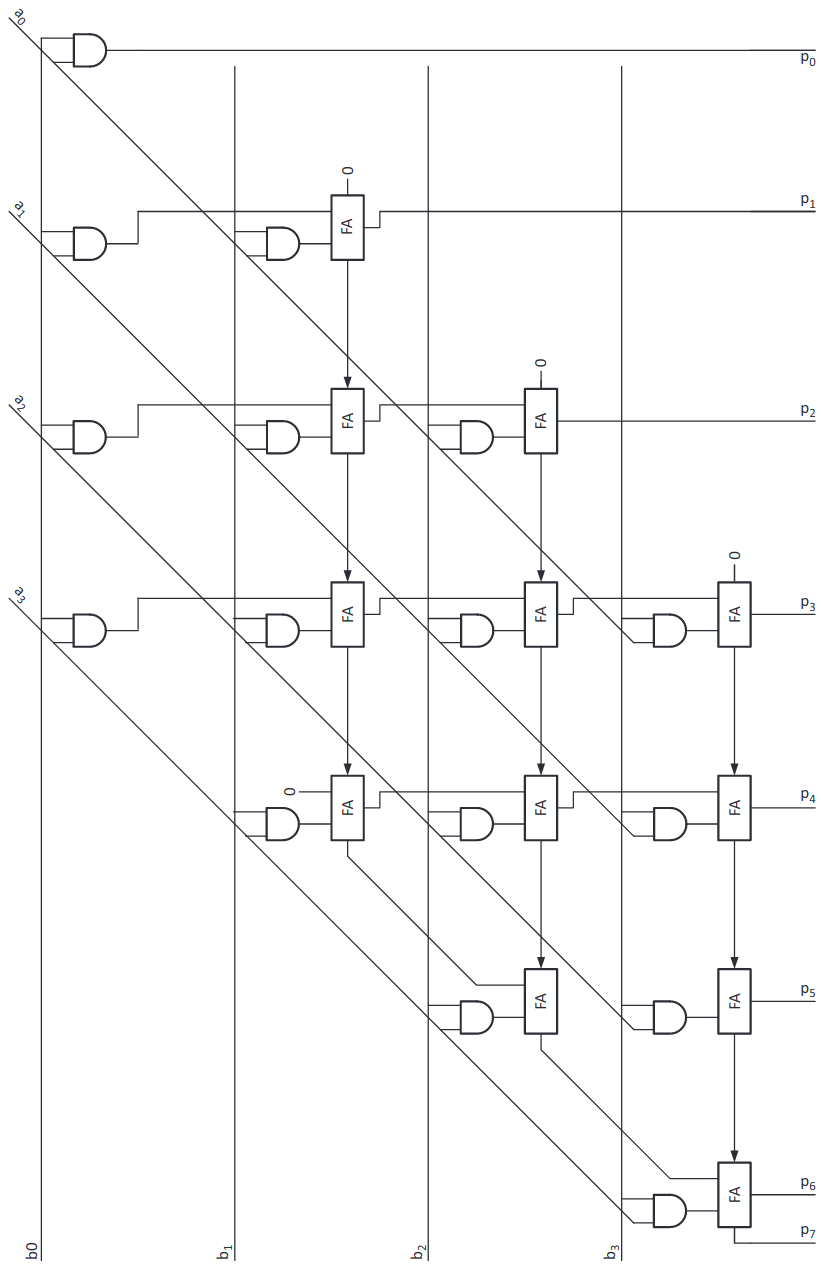
\includegraphics[width=.4\textwidth, origin=c, angle=270]{MultFA.png}
    \caption{8-Bit Multiplier using Full Adders \cite{dally}}
    \label{fig:mult_fa}
\end{figure} 

The multiplier achieves all the steps previously described.
Initially, multiplication occurs using AND gates, then all the inputs get shifted over, as can be seen by the AND gates moving down and the diagonal lines for the A input.
The products are then added with products from the next shifted row down.
This continues, ensuring the carry term also gets forwarded appropriately until the output is achieved.

\subsubsection{State Machine Multiplier}

For this assignment however the combinational design was not used, 
instead, a sequential style of multiplier was provided which is clocked and relies on a Moore state machine to control shifting and adding.
Unlike combinational circuits, which rely only on the current state of the input, sequential designs use feedback to store information about previous inputs\cite{dally}.
In this case, the given circuit is also synchronous meaning that any storage is linked to a clock to ensure all changes happen simultaneously and that races do not occur.
Being both sequential and synchronous makes the circuit a Finite-State Machine\cite{dally}.
Figure \ref{fig:4bit_mult} shows this alternative multiplier design. 

\begin{figure}[H]        
    \centering
    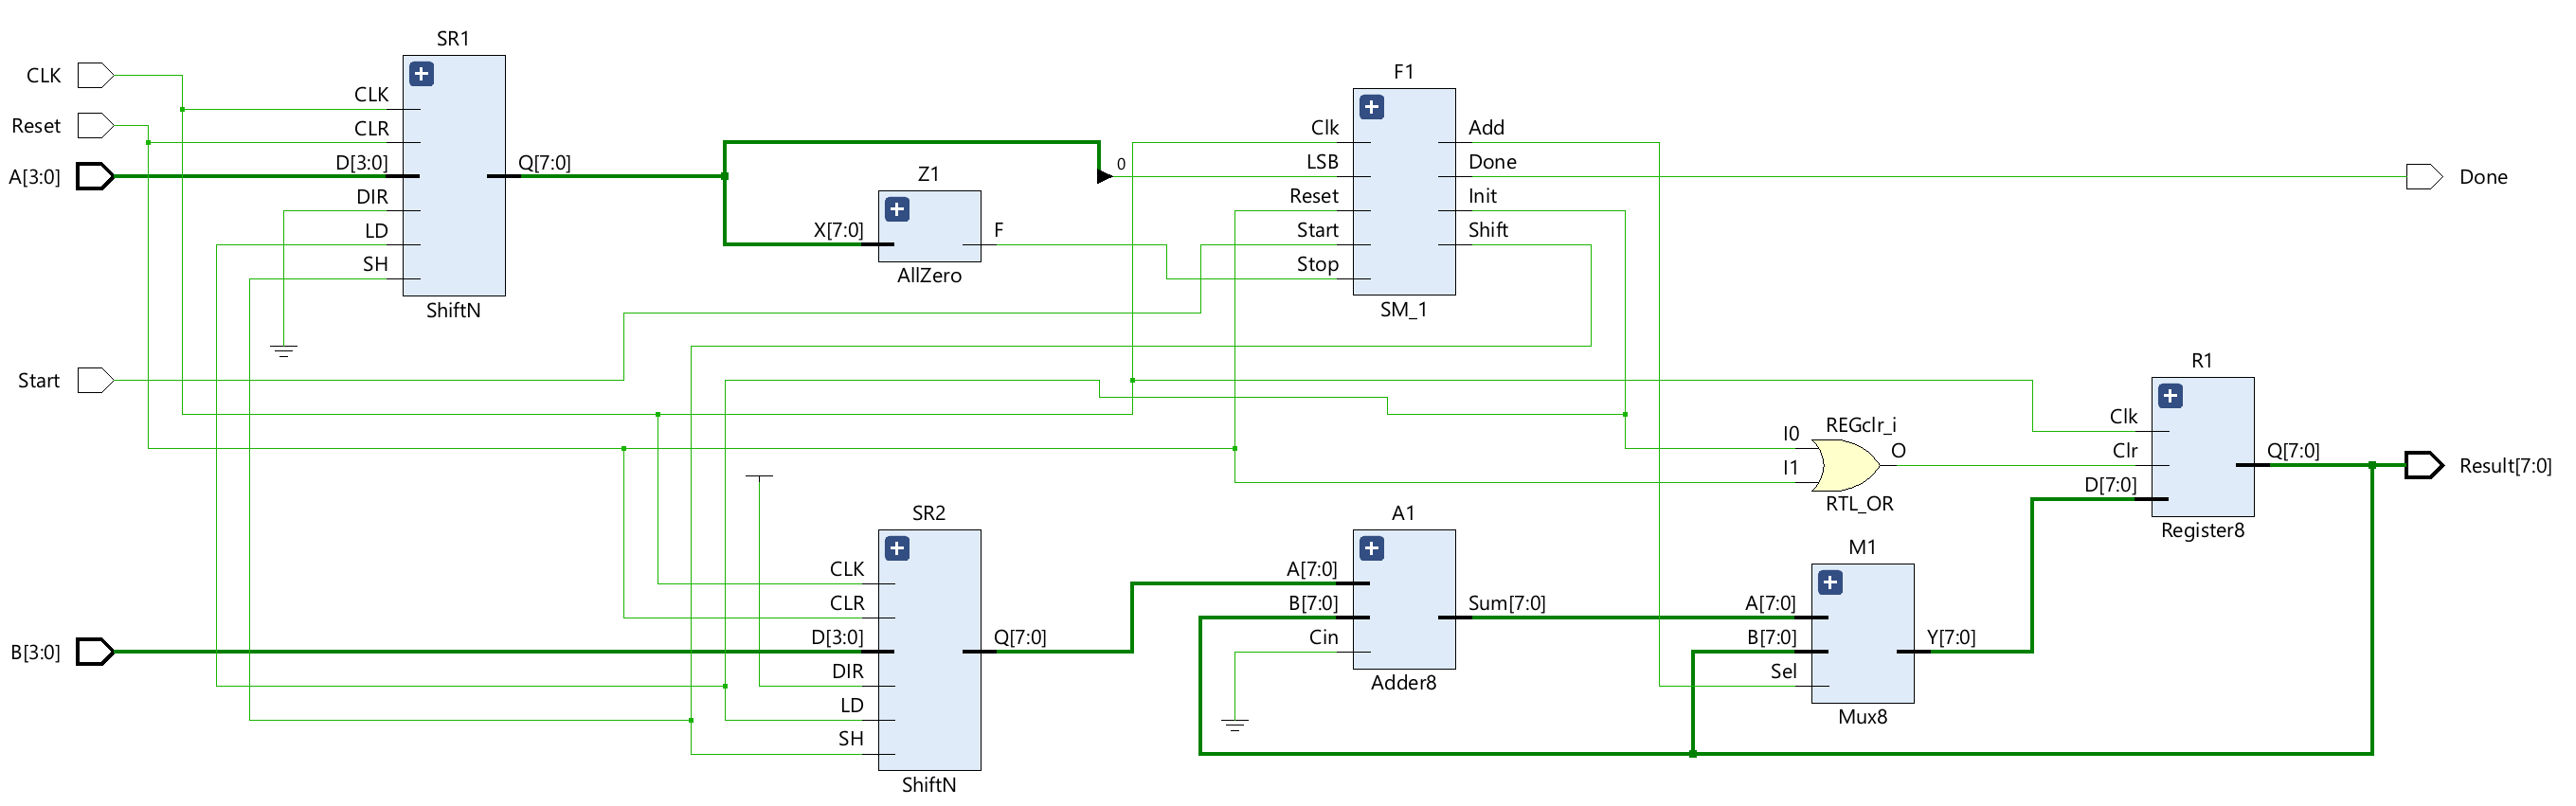
\includegraphics[width=\textwidth]{8bit.png}
    \caption{8-Bit Multiplier using State Machine}
    \label{fig:4bit_mult}
\end{figure} 

F1, the state machine, is at the core of this design, and to understand the multiplier the operation of the state machine must be understood.
One way to visualize a state machine is with a state diagram, such as the one in figure \ref{fig:msm} which is based on the design in \cite{smith1997application}.
Figures \ref{fig:4bit_mult} and \ref{fig:msm} should be referenced will be explained in detail in the remainder of this section and referring back to them can aid with understanding the various stages of the multiplier.

\begin{figure}[H]        
    \centering
    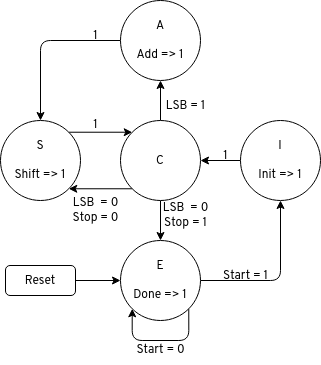
\includegraphics[width=.33\textwidth]{StateMachine.png}
    \caption{Moore State Machine for Multiplier}
    \label{fig:msm}
\end{figure} 

Upon reset, the state machine will always enter state E,
this is the only asynchronous part of the design as this state change will happen as soon as the reset lines goes to '1' while every other state change will only occur on the rising edge of the clock.
In state E the state machine will output '1' on the Done line (any output not labeled as going to '1' is assumed to go to '0') which does not impact any of the other components and is instead an output of the multiplier.
As shown in the diagram while in state E every clock the start signal is checked, as long as it is '0' the state machine remains in state E however once it is '1' it moves to state I.

State I takes the Init line to '1', when tracing this line in figure \ref{fig:4bit_mult} it shows that the following events will occur simultaneously: OR gate REGclr is given an input meaning the gate's output will go to '1' clearing the register of any previous values on the next rising edge.
Note that this will also happen when the Reset line goes '1' as the Reset line connects to the other input of the OR gate. 
The Init line also connects to the LD of both shift registers causing inputs A and B to load into shift registers SR1 and SR2 respectively on the next rising edge.
From state I the state machine will always transition to state C. 

In state C the machine "checks" the value of shift register SR1,
specifically, it checks if all the bits of SR1's output bus are zero (which is sent by the all zero detect Z1 into the stop line), as well as the value of the shift register's least significant bit (LSB).
If the LSB bit is '1' the state moves to the A state, otherwise, the stop line is checked.
When the stop line and LSB bit are '0' the S state is selected and if the stop line is '1' and the LSB is '0' the state returns to the E state.

When in the A state the Add lines goes to '1', which will make the multiplexer M1 select the output of adder A1 instead of the output of register R1.
R1 holds the output value meaning that when the Add line is '0' and M1 feeds R1 back into R1 (causing no change), however when R1 is '1' the output of A1 will go into R1.
A1 adds the output of SR2 together with R1.

State A will always transition to state S which takes the Shift line to '1', causing both SR1 and SR2 to shift with SR1 shifting right as DIR is taken to '0' and SR2 shifting left as DIR is taken high.
Then state S will transition to state C.

These three states (C, A, and S) are the core of the multiplying operation and mirror the steps outlined earlier for multiplying binary numbers.
As mentioned earlier, instead of directly multiplying two 4-bit numbers this state machine break the multiplication into multiple 4-bit by 1-bit multiplications.
For any N-bit ($n$) by 1-bit ($b$) multiplication the following holds: $n \times b = n$ if $b = 1$ or $n \times b = 0$ if $b = 0$.
So the way the state machine multiplies two multi-bit binary numbers ($A$ and $B$) is to add a shifted copy of $B$ to the register for every position $A$ is 1\cite{dally}. 

With the state machine and all other components now covered, the next stage of this assignment was to test and verify the 8-bit multiplier design.

\subsection{Test Bench}
The provided test bench code for the 8-bit multiplier was used with some minor changes and corrections.
The initially provided code used SRA as a variable name which is invalid VHDL code as SRA is in the reserved list,
this however is a simple fix as the variable can be renamed throughout the test bench.
The test approach taken in the original test bench was to iterate a 2D array testing a range of numbers for A for a range of numbers of B.
These integers when then converted to busses and connected to the multiplier, with the multiplier's output being converted into an integer.
To make the test bench more thorough the range of values investigated was increased to cover every possible 4-bit input (0 to 15) of A for every possible 4-bit number of B, instead of the original limited range.
This made finding errors more complicated however due to a large amount of values output so another signal was added that keeps a running total of the number of errors.
The error checking is done with an if statement that calculates the product of the integers going into the multiplier and compares it to the output of the multiplier.
If the values do not match an error is logged and the error count is incremented. 
Keeping track of errors helped during debugging to ensure that the multiplier functioned as expected. 

\begin{figure}        
    \centering
    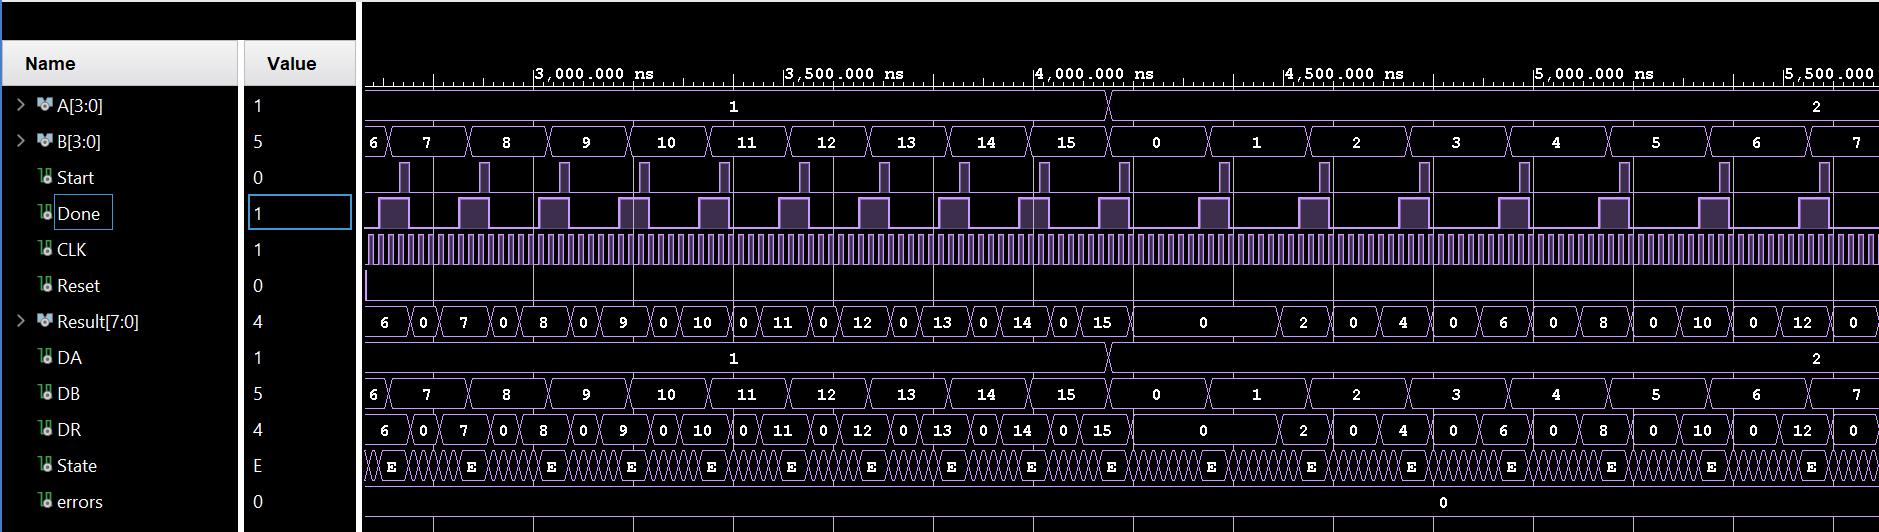
\includegraphics[width=\textwidth]{8bit_test.png}
    \caption{Test Bench of 8-Bit Multiplier}
    \label{fig:4bit_testbench}
\end{figure} 

Comprehensive testing, a snippet of which can be seen in figure \ref{fig:4bit_testbench}, such as this ensures that the multiplier will work as expected in every single case.
The top six rows shows all the inputs and outputs of the multiplier, with Done and Result being the only outputs, as well as some additional information below such as the state of the state machine and the error count.
Having this information available makes it easier to confirm each use case by looking at the values of A, B, and Result at the rising edge of each Done.
Indeed after the minor correction to the test bench this design simulated every combination of inputs with no errors logged.

\subsection{Timing Analysis}

The worst-case timing of the 8-bit multiplier can be found by delving into the state machine. 
This is because timing is dictated by the number of clock cycles, with each full clock cycle being 20ns, and the state machine will dictate how many clock cycles multiplication takes.
Referring to the diagram in figure \ref{fig:msm} the shortest complete journey occurs when the state go from $E \rightarrow I \rightarrow C \rightarrow E$, which occurs anytime A is $A = 0_{16}$ regardless of the value of B.
This would take only 60ns from the start input to the done output.
The longest journey will occur if the multiplier needs to add and shift for every single bit of A, ie when $A = F_{16}$, this is once again independent of the value of B.
In this case, it would go $E \rightarrow I \rightarrow C \rightarrow A \rightarrow S \rightarrow C \rightarrow A \rightarrow S \rightarrow C \rightarrow A \rightarrow S \rightarrow C \rightarrow A \rightarrow S \rightarrow C \rightarrow E$.
This would take 300ns from start to done, which can be confirmed in simulation as seen in figure \ref{fig:4bit_worstcase}.

\begin{figure}[H]        
    \centering
    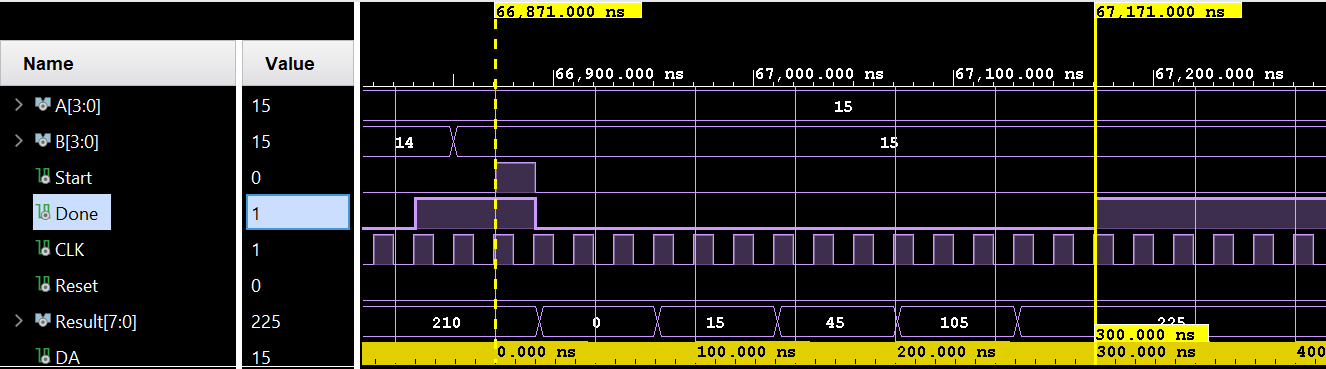
\includegraphics[width=\textwidth]{8bit_worst.png}
    \caption{Worst Case performance of 8-Bit Multiplier}
    \label{fig:4bit_worstcase}
\end{figure} 

The average execution time can also be calculated based on the states given a uniform distribution of values of A. 
While a mathematical proof is possible, for this report all possible values of A and the number of clock cycles taken were simulated using python code (see appendix)
which revealed the average number of clock cycles is 11.125, which would give an execution time, on average, of 222.5 ns.
Below is a bar graph, figure \ref{fig:bar}, of all possible clock cycles times per value of A.
This shows how timing generally gets worse with larger values as it takes longer to get the all zero signal and more adds and shifts need to occur.
Of note is the fact that larger numbers are not always slower as 11 takes longer than 12, the reason for this is made clear when looking at the the binary representations (1011 and 1100)
as both will need to shift four times but the smaller number will actually need an additional add over the larger.

\begin{figure}[H]        
    \centering
    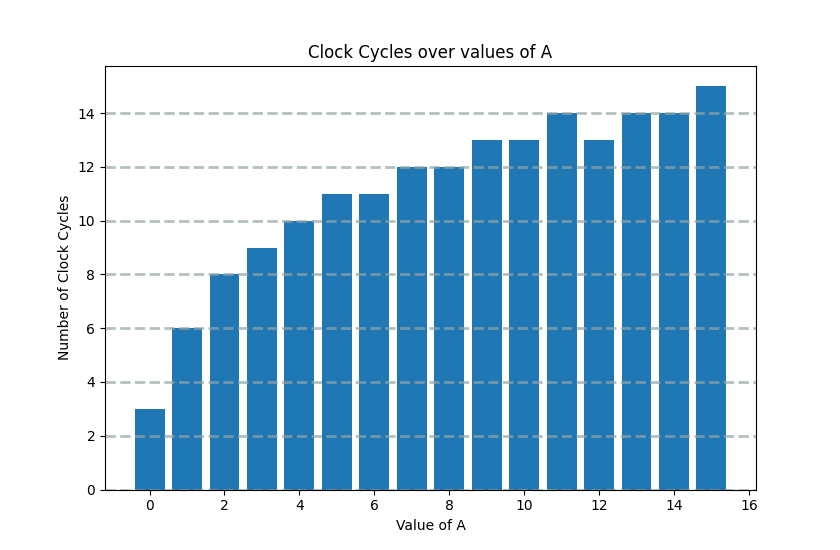
\includegraphics[width=.75\textwidth]{ClockCycles.png}
    \caption{Bar Graph of all Clock Cycles}
    \label{fig:bar}
\end{figure} 

\section{8-Bit Multiplier}

8-Bit multipliers can be constructed in various methods, one simple example would be expanding the design seen in figure \ref{fig:mult_fa} to take 8-bit inputs and to extend the shift-registers, register, multiplexer and adder in figure \ref{fig:4bit_mult}.
These methods however go against some VHDL good practices (as well as against the assignment's instructions),
as it is preferred to have smaller components that can be reused throughout a design.

\subsection{Theory}

For this assignment, the 8-bit multiplier was used as a component, alongside additional 8-bit adders. 
This is because 16-bit multiplication can be described as four separate 8-bit multiplication.
Take for example the multiplication of $49_16$ and $9D_16$ in equation \ref{eq:16bit} below.

\begin{equation}
    \label{eq:16bit}
    \begin{tabular}{c c c c c c c c c c c c c c c c c c}
        &   &   &   &   &  &  &  &   & 0 & 1 & 0 & 0 & 1 & 0 & 0 & 1\\
        &   &   &   & &&&&$\times$   & 1 & 0 & 0 & 1 & 1 & 1 & 0 & 1 \\
                \hline
        &   &   &   &   &   &   &   &   & \hlc[cyan]{0} & \hlc[cyan]{1} & \hlc[cyan]{0} & \hlc[cyan]{0} & \hlc[yellow]{1} & \hlc[yellow]{0} & \hlc[yellow]{0} & \hlc[yellow]{1} \\
        &   &   &   &   &   &   &   & \hlc[cyan]{0} & \hlc[cyan]{0} & \hlc[cyan]{0} & \hlc[cyan]{0} & \hlc[yellow]{0} & \hlc[yellow]{0} & \hlc[yellow]{0} & \hlc[yellow]{0} &   \\
        &   &   &   &   &   &   & \hlc[cyan]{0} & \hlc[cyan]{1} & \hlc[cyan]{0} & \hlc[cyan]{0} & \hlc[yellow]{1} & \hlc[yellow]{0} & \hlc[yellow]{0} & \hlc[yellow]{1} &   &   \\
        &   &   &   &   &   & \hlc[cyan]{0} & \hlc[cyan]{1} & \hlc[cyan]{0} & \hlc[cyan]{0} & \hlc[yellow]{1} & \hlc[yellow]{0} & \hlc[yellow]{0} & \hlc[yellow]{1} &   &   &   \\
        &   &   &   &   & \hlc[green]{0} & \hlc[green]{1} & \hlc[green]{0} & \hlc[green]{0} & \hlc[pink]{1} & \hlc[pink]{0} & \hlc[pink]{0} & \hlc[pink]{1} &   &   &   &   \\
        &   &   &   & \hlc[green]{0} & \hlc[green]{0} & \hlc[green]{0} & \hlc[green]{0} & \hlc[pink]{0} & \hlc[pink]{0} & \hlc[pink]{0} & \hlc[pink]{0} &   &   &   &   &   \\
        &   &   & \hlc[green]{0} & \hlc[green]{0} & \hlc[green]{0} & \hlc[green]{0} & \hlc[pink]{0} & \hlc[pink]{0} & \hlc[pink]{0} & \hlc[pink]{0} &   &   &   &   &   &   \\
        &   & \hlc[green]{0} & \hlc[green]{1} & \hlc[green]{0} & \hlc[green]{0} & \hlc[pink]{1} & \hlc[pink]{0} & \hlc[pink]{0} & \hlc[pink]{1} &   &   &   &   &   &   &   \\
                \hline
        & 0 & 0 & 1 & 0 & 1 & 1 & 0 & 0 & 1 & 1 & 0 & 0 & 0 & 1 & 0 & 1 \\
    \end{tabular} 
\end{equation}

As shown by the colors this can be broken down into the following four 4-bit multiplications. 
\vspace{5mm}
\begin{minipage}{.5\linewidth}
    \begin{equation}
        \label{eq:yellow}
        \begin{tabular}{c c c c c c c c c }
            &   &   &   &   & 1 & 0 & 0 & 1 \\
            &   &   &   &  $\times$ & 1 & 1 & 0 & 1 \\
            \hline
            &   &   &   &   & 1 & 0 & 0 & 1 \\
            &   &   &   & 0 & 0 & 0 & 0 &   \\
            &   &   & 1 & 0 & 0 & 1 &   &   \\
            &   & 1 & 0 & 0 & 1 &   &   &   \\
            \hline
            & \hlc[yellow]{0} & \hlc[yellow]{1} & \hlc[yellow]{1} & \hlc[yellow]{1} & \hlc[yellow]{0} & \hlc[yellow]{1} & \hlc[yellow]{0} & \hlc[yellow]{1} \\
        \end{tabular} 
    \end{equation}
    \end{minipage}%
    \begin{minipage}{.5\linewidth}
        \begin{equation}
            \label{eq:blue}
            \begin{tabular}{c c c c c c c c c }
                &   &   &   &   & 0 & 1 & 0 & 0 \\
                &   &   &   &  $\times$ & 1 & 1 & 0 & 1 \\
                \hline
                &   &   &   &   & 0 & 1 & 0 & 0 \\
                &   &   &   & 0 & 0 & 0 & 0 &   \\
                &   &   & 0 & 1 & 0 & 0 &   &   \\
                &   & 0 & 1 & 0 & 0 &   &   &   \\
                \hline
                & \hlc[cyan]{0} & \hlc[cyan]{0} & \hlc[cyan]{1} & \hlc[cyan]{1} & \hlc[cyan]{0} & \hlc[cyan]{1} & \hlc[cyan]{0} & \hlc[cyan]{0} \\
            \end{tabular} 
        \end{equation}
\end{minipage}
\vspace{5mm}
\begin{minipage}{.5\linewidth}
    \begin{equation}
        \label{eq:pink}
        \begin{tabular}{c c c c c c c c c }
            &   &   &   &   & 1 & 0 & 0 & 1 \\
            &   &   &   &  $\times$ & 1 & 0 & 0 & 1 \\
            \hline
            &   &   &   &   & 1 & 0 & 0 & 1 \\
            &   &   &   & 0 & 0 & 0 & 0 &   \\
            &   &   & 0 & 0 & 0 & 0 &   &   \\
            &   & 1 & 0 & 0 & 1 &   &   &   \\
            \hline
            & \hlc[pink]{0} & \hlc[pink]{1} & \hlc[pink]{0} & \hlc[pink]{1} & \hlc[pink]{0} & \hlc[pink]{0} & \hlc[pink]{0} & \hlc[pink]{1} \\
        \end{tabular} 
    \end{equation}
    \end{minipage}%
    \begin{minipage}{.5\linewidth}
        \begin{equation}
            \label{eq:green}
            \begin{tabular}{c c c c c c c c c }
                &   &   &   &   & 0 & 1 & 0 & 0 \\
                &   &   &   &  $\times$ & 1 & 0 & 0 & 1 \\
                \hline
                &   &   &   &   & 0 & 1 & 0 & 0 \\
                &   &   &   & 0 & 0 & 0 & 0 &   \\
                &   &   & 0 & 0 & 0 & 0 &   &   \\
                &   & 0 & 1 & 0 & 0 &   &   &   \\
                \hline
                & \hlc[green]{0} & \hlc[green]{0} & \hlc[green]{1} & \hlc[green]{0} & \hlc[green]{0} & \hlc[green]{1} & \hlc[green]{0} & \hlc[green]{0} \\
            \end{tabular} 
        \end{equation}
\end{minipage}

The products of these multipliers can then be added together as seen in equation \ref{eq:16bit_add} to get the same result as equation \ref{eq:16bit}.
This addition can be achieved with three 16-bit adders, which could be constructed out of six of the provided 8-bit adders.

\begin{equation}
    \label{eq:16bit_add}
    \begin{tabular}{c c c c c c c c c c c c c c c c c c}
        &   &   &   &   &   &   &   & \hlc[yellow]{0} & \hlc[yellow]{1} & \hlc[yellow]{1} & \hlc[yellow]{1} & \hlc[yellow]{0} & \hlc[yellow]{1} & \hlc[yellow]{0} & \hlc[yellow]{1} & \\
        &   &   &   &  \hlc[cyan]{0} & \hlc[cyan]{0} & \hlc[cyan]{1} & \hlc[cyan]{1} & \hlc[cyan]{0} & \hlc[cyan]{1} & \hlc[cyan]{0} & \hlc[cyan]{0}&   &   &   &   &   &\\
        &   &   &   &  \hlc[pink]{0} & \hlc[pink]{1} & \hlc[pink]{0} & \hlc[pink]{1} & \hlc[pink]{0} & \hlc[pink]{0} & \hlc[pink]{0} & \hlc[pink]{1}&  &   &   &   &   \\
        \hlc[green]{0} & \hlc[green]{0} & \hlc[green]{1} & \hlc[green]{0} & \hlc[green]{0} & \hlc[green]{1} & \hlc[green]{0} & \hlc[green]{0}  &   &   &  &   &   &   &   \\
        \hline
        0 & 0 & 1 & 0 & 1 & 1 & 0 & 0 & 1 & 1 & 0 & 0 & 0 & 1 & 0 & 1 & \\

    \end{tabular} 
\end{equation}

\begin{equation}
    \label{eq:16bit_add1}
    \begin{tabular}{c c c c c c c c c }
                &   &   &   &   & \hlc[yellow]{0} & \hlc[yellow]{1} & \hlc[yellow]{1} & \hlc[yellow]{1} \\
            +   & \hlc[cyan]{0} & \hlc[cyan]{0} & \hlc[cyan]{1} & \hlc[cyan]{1} & \hlc[cyan]{0} & \hlc[cyan]{1} & \hlc[cyan]{0} & \hlc[cyan]{0} \\
                \hline
                & 0 & 0 & 1 & 1 & 1 & 0 & 1 & 1 \\
    \end{tabular} 
\end{equation}

\begin{equation}
    \label{eq:16bit_add2}
    \begin{tabular}{c c c c c c c c c c}
                & 0 & 0 & 1 & 1 & 1 & 0 & 1 & 1 \\
               + & \hlc[pink]{0} & \hlc[pink]{1} & \hlc[pink]{0} & \hlc[pink]{1} & \hlc[pink]{0} & \hlc[pink]{0} & \hlc[pink]{0} & \hlc[pink]{1} \\
                \hline
               0 & 1 & 0 & 0 & 0 & 1 & 1 & 0 & 0 \\
    \end{tabular} 
\end{equation}

\begin{equation}
    \label{eq:16bit_add3}
    \begin{tabular}{c c c c c c c c c }
                &   &   &   & 0 & 1 & 0 & 0 & 0 \\
            +   & \hlc[green]{0} & \hlc[green]{0} & \hlc[green]{1} & \hlc[green]{0} & \hlc[green]{0} & \hlc[green]{1} & \hlc[green]{0} & \hlc[green]{0} \\
                \hline
                & 0 & 0 & 1 & 0 & 1 & 1 & 0 & 0 \\
    \end{tabular} 
\end{equation}

However a more efficient design can be created as each of these inputs can be considered as "shifted" 8-bit values,
this design makes use of only three 8-bit adders and the operation behind it can be seen in equations \ref{eq:16bit_add1},  \ref{eq:16bit_add2}, and  \ref{eq:16bit_add3}.

Equation \ref{eq:16bit_add} shows how the 3 down to 0 bits of the yellow (\ref{eq:yellow}) multiplier's output can be passed directly into the 3 down to 0 bits of the final results.
The 7 down to 4 bits of this output however have to be summed with the output of the blue (\ref{eq:blue}), but these cannot be directly added as the upper yellow bits have to be shifted down.
This shift can be achieved by wiring the 7 to 4 bits of the yellow to 3 down to 0 inputs of the adder's input and keeping the other bits at '0'.
The output of this first adder can then be fed into the next adder along with the pink (\ref{eq:pink}) multiplier product to get the next step as seen in equation \ref{eq:16bit_add2}.
Once more the 3 down to 0 bits can be passed to the final result (the 7 down to 4 bits) and then the 'shifting' can be employed once more to shift the 7 down to 4 bits into the 3 down to 0 bits of the next adder's input.
Those shifted bits along with the final green multiplier output can be added together in the final third adder as seen in equation \ref{eq:16bit_add3} to product the last 8 bits of the result.

Doing so introduces a few edge cases however as adders also output a carry line. 
For adder 1 the carry can be ignored as the largest output of an 8-bit multiplier is $E1_{16}$,
and accounting for the shift, the largest values the adder will encounter are $0E_{16} + E1_{16}$ for which the output is $EF_{16}$. 
$EF_{16}$ can be conveyed as an 8-bit number meaning the carry will always be '0'.
This however is not true for the adder 2 (\ref{eq:16bit_add2}) where the largest possible sum is $EF_{16} + E1_{16} = 1D0_{16}$, which means the carry line may go to '1'.
Adder 2's carry, therefore, needs to be propagated, which can be done by connecting it to bit 4 of adder 3's input,
specifically, the input with the down-shifted number as bits 7 to 4 will always go unused otherwise.
Adder 3's carry will also always be '0' as the largest possible values to enter this adder would be $1D_{16} + E1_{16} = FE_{16}$, once more a number that can be conveyed in 8-bits.
With all of these steps, a 16-bit Multiplier can be constructed out of four 8-bit multipliers and three 8-bit adders. 


\begin{figure}[H]         
    \centering
    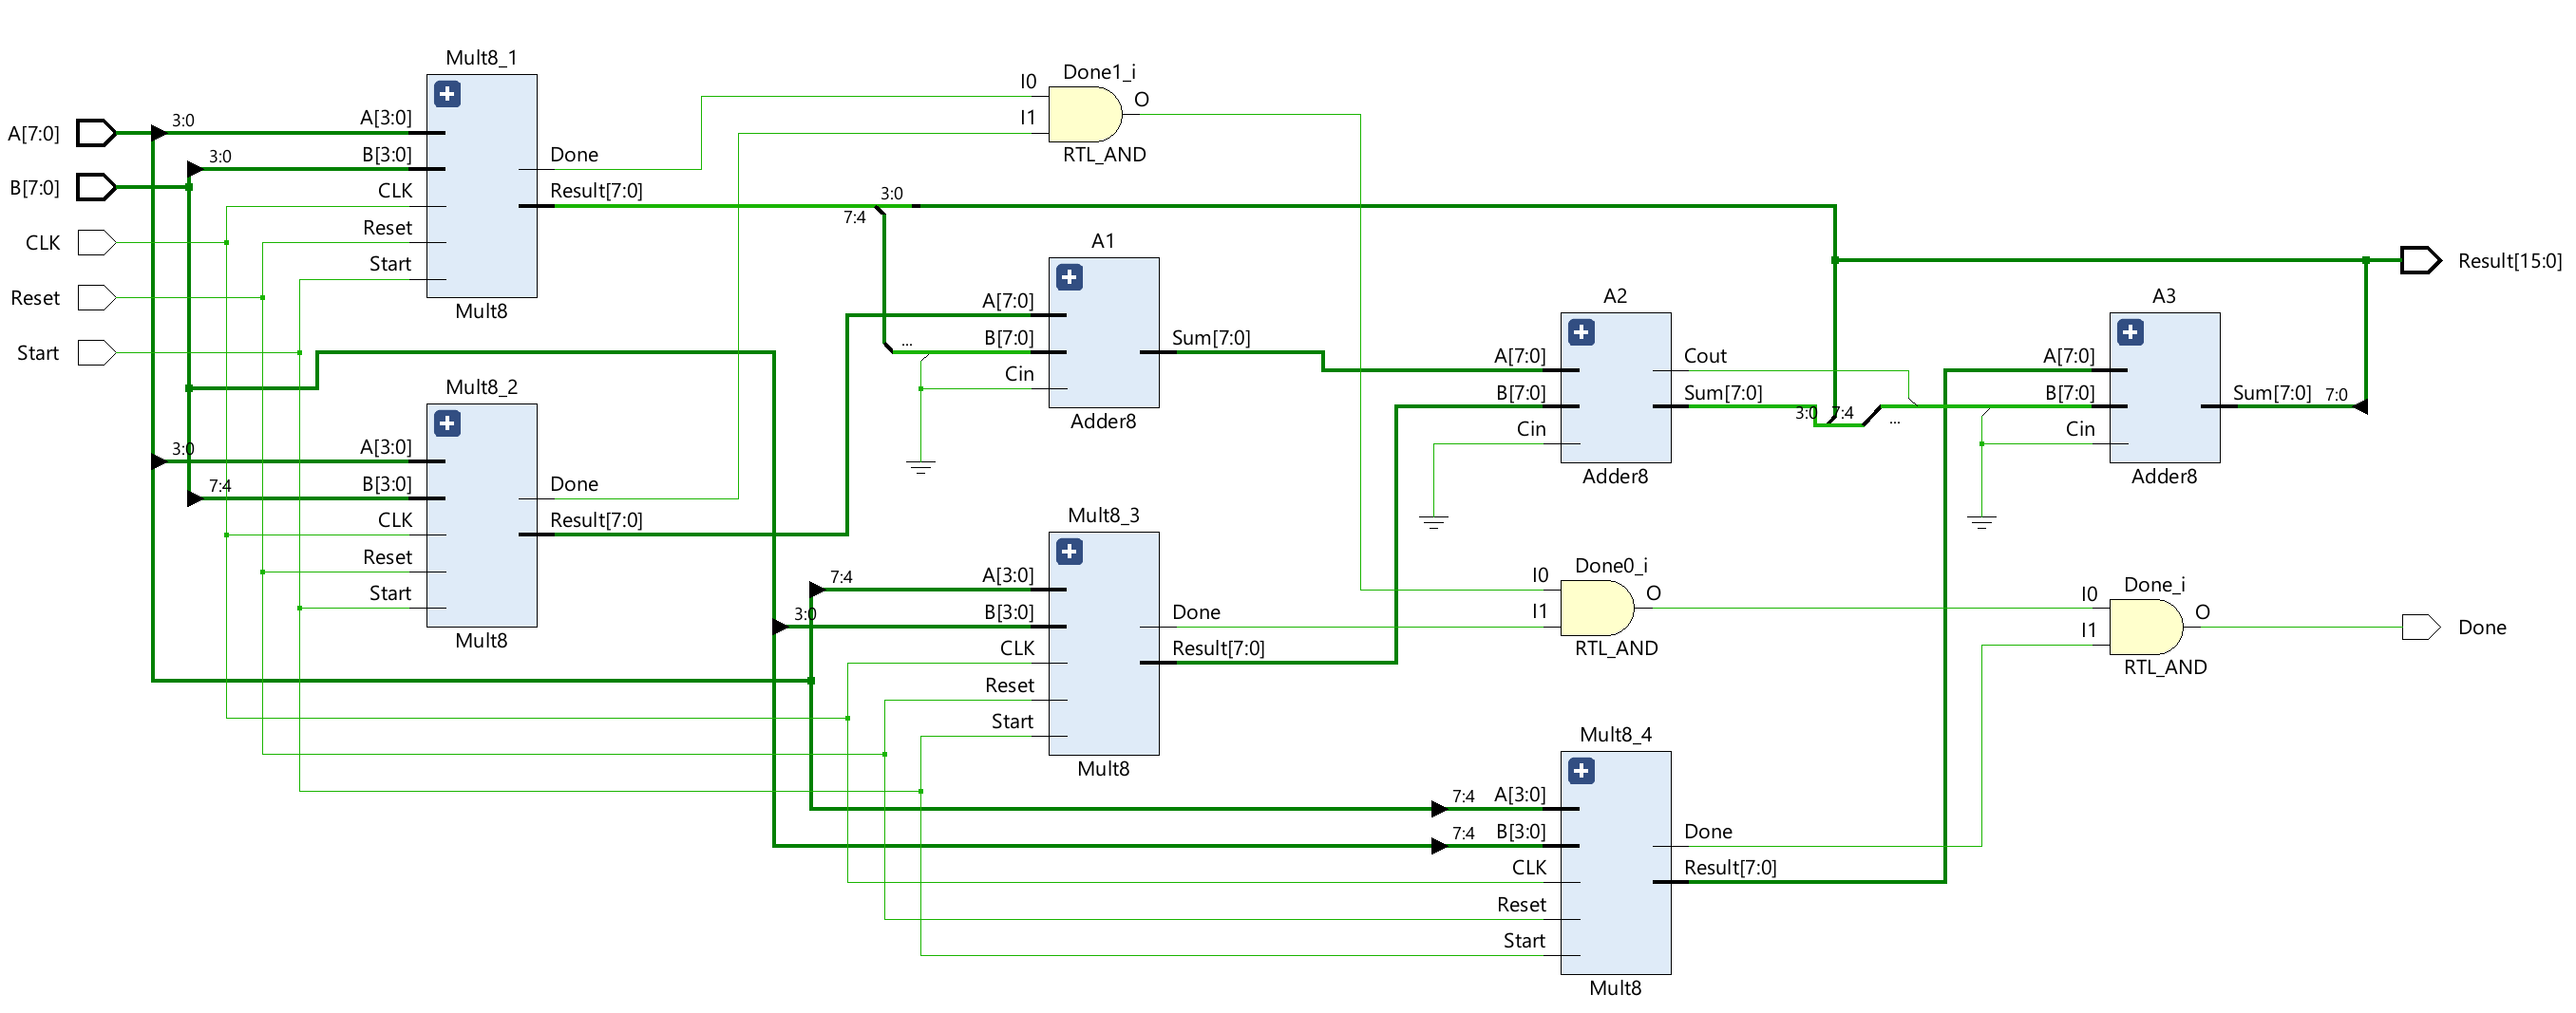
\includegraphics[width=\textwidth]{16bit.png}
    \caption{16-Bit Multiplier}
    \label{fig:8bit}
\end{figure} 

The final 16-bit multiplier design can be seen in figure \ref{fig:8bit},
note that the inputs and outputs mirror that of the original 8-bit multiplier with a clock, reset, and start going in alongside two 8-bit values and a single 16-bit output with a done line.
All inputs are connected to the inputs of the 8-bit multipliers within, with the A and B lines being split as described earlier. 
The output consists of the result obtained by following equation \ref{eq:16bit_add} and the done line waiting for all four multipliers to have output on their done line.
An older version of the design also included two 8-bit registers to hold the result just as with the 8-bit design, however, these were removed as they served no purpose in this larger 16-bit design.
While in the 8-bit design, the temporary value of the result is needed in the calculation, this is not the case in the 16-bit design and there is no benefit in storing these values besides ensuring the value is held constant between rising edges of clocks.
If the 16-bit multiplier however made use of different clock cycles for each component having a final register in sync with the main clock would be beneficial.

After creating this design and researching for this report it was discovered that this simple combination of 7 components and a few extra logic gates is also known as a Vedic multiplier \cite{vedic}.
The method is based on a traditional ancient Indian technique for fast multiplication and is often used in digital signal processing due to this speed.
While this design is faster, it is also more complex and takes up more space than other types of multipliers.

\subsection{Test Bench}
Extending the previous test bench from the 8-bit multiplier to this design was simple,
as care was taken to ensure the 16-bit multiplier had the same inputs and outputs as the 8-bit multiplier.
So the original code was extended to input all numbers from 0 to 255 on both ports and the same error count signal was used to aid with early debugging and verification.
Initial testing showed errors at the A input 252, which is binary '11111100', this is also the first instance where the carry bit should be influencing the outcome.
Using the error signal it was easy to find all the spots with problems and confirm indeed that the carry was an issue,
then comparing the VHDL code to the design revealed that indeed the carry had not been connected properly.

Another note with this test bench as compared to the previous one is that execution time is far longer.
While Vivado allowed the default simulation time to be set to 20ms making the simulation of all values simple.
Simulating this much took far longer than the previous simulations for 8-bit however, and this shows how comprehensive testing will eventually cease to be an option for more complicated applications once there are too many possible inputs to test and confirm them all.

\subsection{Timing Analysis}
Timing for this multiplier was simpler, as there are no synchronous elements introduced besides the 8-bit multiplier and the adders will complete well before the end of the clock cycle.
Therefore the worst-case execution time is as long as the longest 8-bit multiplication.
As discussed before the 8-bit multiplier is fully dependent on the A input for its timing with $F_{16}$ being the worst-case.
As the new longer A input is split into two, the worst-case timing will now occur when either half is $F_{16}$, ie when $A = XF_{16}$ or $A = XF_{16}$ (where $X$ is any hex digit) regardless of B.
This path can be seen being measured in figure \ref{fig:8bit_worst} and is still 300ns or 15 clock cycles.

\begin{figure}[H]         
    \centering
    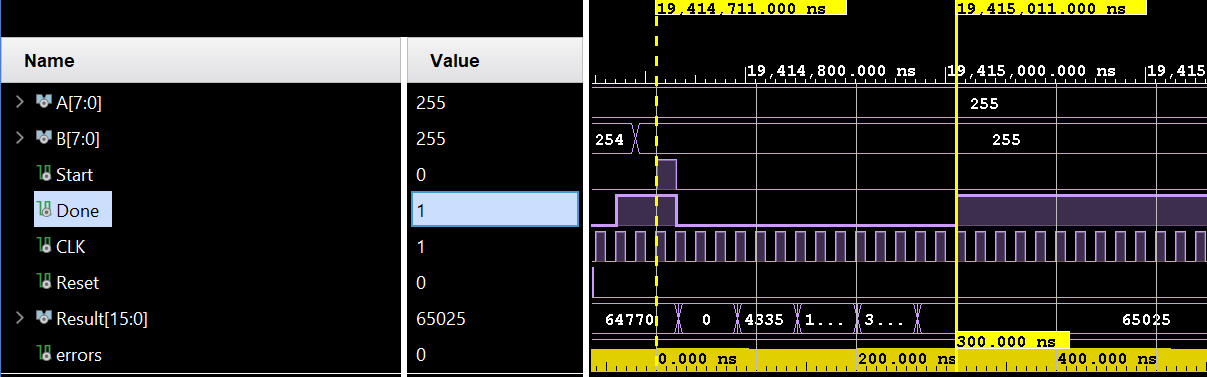
\includegraphics[width=\textwidth]{16bit_worst.png}
    \caption{16-Bit Multiplier Worst-Case Execution Time}
    \label{fig:8bit_worst}
\end{figure} 

The best case time is therefore when $A=00_{16}$ with 60ns.
Average timing therefore also changes, and when calculated with the code in the appendix comes out to 12.8125 clocks or 256.25ns.
This is because the execution time is limited by the worst case of either half of A, meaning the average will be higher than before.

While the number of clock cycles required in this design cannot be reduced the length of each clock cycle can be.
As timings were given for every single component the amount of time needed within each clock cycle to complete the longest possible operation can be calculated,
this was attempted for this report and ultimately it was discovered that the clock could be taken from 20ns to 3ns.
This reduces the timings significantly however caution is required as these timings may work only in simulation and a more accurate timing report would need to consider the paths between components on the silicon.

\section{Conclusion and Improvements}
This report has covered the theory and testing of both an 8-bit and 16-bit multiplier design,
touching on different design philosophies and timing. 
Doing so has provided valuable hands-on experience in VHDL and in particular with using Vivado.

Earlier sections covering theory spoke of some improvement, but this final section will outline some more possible improvements.
These "improvements" always come with another cost, meaning the ultimate decision will depend on the use case.
As mentioned before the designs used in this report are not the only option for multipliers, in particular, the 8-bit multiplier could make use of the combinational design mentioned earlier.
The combinational design however does not guarantee results on a clock cycle as the current design does,
however by adding registers to store the inputs and output as well as a simplified state machine the benefits of getting results on a certain clock cycle can be combined with the speed of the combinational design.
Another method to increase execution time, besides the aforementioned increases in clock speed, would be to optimize the value used for the A inputs of the 8-bit finite state machine design.
This is because, as seen in figure \ref{fig:bar}, the execution time is linked to the A and generally a smaller value will be faster to compute. 
Knowing this about the multiplier component would be useful as a design that incorporate should take care to use try and route the smaller of the two numbers into A.
Logic could also be added to ensure A is the smaller value, this however is complicated as it may nullify any speed benefits and will certainly have a cost in terms of area and power. 
For the 16-bit multiplier, the main improvements consist of improving the 8-bit multiplier with-in, as the design is limited by those.
Another improvement would be to replace the ripple adders with look ahead adders, which are more complex and larger but can speed up adding.
These speed improvements however are useless unless the goal is also to reduce the clock lengths.

\pagebreak
\appendix
\section{Python Code 8-bit} 
\begin{lstlisting}
    import math
    total_num_clock = 0
    
    values = range(0,16)
    num_clocks = []
    
    for value in values:
        num_clock = 2 # From E to I
        bin = f'{value:08b}'
        print(bin)
        for char in bin[::-1]:
            num_clock += 1 # For C
            if value == 0:
                break
            if char == '1':
                num_clock += 1 # For A
            value = math.floor(value/2)
            num_clock += 1 # For S
        print(num_clock)
        total_num_clock += num_clock
        num_clocks.append(num_clock)
    
    average_num_clock = total_num_clock / 16
    print(average_num_clock)
\end{lstlisting}

\section{Python Code 16-bit} 
\begin{lstlisting}
import math
total_num_clock = 0

values = range(0,256)
num_clocks = []

def get_clocks(bin):
    bin = '0' + bin
    value = int(bin, 2)
    print(bin)
    num_clock = 2 # From E to I
    for char in bin[::-1]:
        num_clock += 1 # For C
        if value == 0:
            break
        if char == '1':
            num_clock += 1 # For A
        value = math.floor(value/2)
        num_clock += 1 # For S
    return num_clock

for value in values:
    bin = f'{value:08b}'
    print(bin)
    bin_1 = bin[:4]
    bin_2 = bin[4:]
    #print(bin_1)
    #print(bin_2)
    num_clock = max(get_clocks(bin_1), get_clocks(bin_2))
    print(num_clock)
    total_num_clock += num_clock
    num_clocks.append(num_clock)

average_num_clock = total_num_clock / len(num_clocks)
print(average_num_clock)
\end{lstlisting}


\pagebreak
\printbibliography

\end{document}